\documentclass{article}
\usepackage{graphicx} % Required for inserting images
\usepackage{indentfirst}
\usepackage[a4paper, margin=3cm]{geometry}
\usepackage{amssymb}
\usepackage{amsmath}
\usepackage[portuguese]{babel}
\usepackage[breakable]{tcolorbox}
\usepackage[rightcaption]{sidecap}
\usepackage{wrapfig}
\usepackage{caption}
\usepackage{subfig}
\usepackage{hyperref}
\usepackage{xcolor}

    
    \geometry{verbose,tmargin=1in,bmargin=1in,lmargin=1in,rmargin=1in}

\title{Árvore Geradora Mínima}
\author{Kauan Mariani Ferreira, Mariana Fernandes Rocha, Pedro Henrique Coterli}
\date{23 de novembro de 2023}

\begin{document}

\maketitle

\section{Introdução}
A teoria dos grafos é uma área muito ampla da Matemática e surgiu da tentativa de Leonard Euler de resolver o problema de Konnigsberg, em 1736. Dessa forma, um problema da vida real foi o estopim para a criação dessa teoria, que, apesar de parecer abstrata, tem suas origens centradas principalmente na aplicação de problemas da vida real.\\

De modo análogo ao problema enfrentado por Euler, Otakar Borůvka (1899-1995), matemático do século XX, se deparou com um problema numa pequena cidade da República Tcheca. Como encontrar um arranjo para a distribuição da rede elétrica que gere um custo mínimo para a empresa de energia? A empresa estava prestes a montar a rede elétrica na cidade e precisa instalar suas conexões de forma a percorrer todas as casas da cidade com o menor custo possível. Como encontrar um caminho que satisfaça essa propriedade? Como fazer um algoritmo que, dado um grafo, sempre encontre o caminho mínimo? Essa tarefa é possível?\\

De modo a definir o problema para um tratamento um pouco mais formal, podemos enunciá-lo como:
dado um grafo G = (V, E) conexo, não-direcionado e com pesos, em conjunto com a função w: E $\rightarrow \mathbb{R}$, que atribui um peso w(e) $\in \mathbb{R}$ para cada aresta, queremos um algoritmo que minimiza a função:

\begin{center}

\begin{gather*}
    \sum_{v \in E} w(e)
\end{gather*}

\end{center}

A resposta para esse problema é que sim, sempre existe um caminho mínimo, e ao longo da história vários algoritmos foram encontrados para resolver esse problema, muitas das vezes de forma independente. Os algoritmos que iremos tratar hoje são chamado de algoritmos clássicos, pois são algoritmos gananciosos (ou míopes), que procuram a melhor possibilidade de escolha a cada iteração do algoritmo e consequentemente acaba encontrando a melhor possibilidade globamente. Abaixo temos um exemplo de caminho mínimo:\\

\begin{figure}[h]
\centering
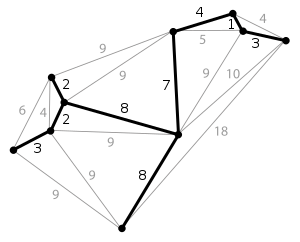
\includegraphics[width = 0.3\textwidth]{Minimum_spanning_tree.svg.png}
\caption{Um grafo e sua árvore de caminho mínimo}
\label{fig:enter-label}
\end{figure}

\section{Propriedades}

Motivados por Borůvka, os estudos sobre as árvores geradoras mínimas desempenham um papel crucial em uma variedade de aplicações práticas, sendo também fundamental conhecer suas propriedades e condições necessárias e suficientes, que serão ilustradas nesta seção.

\subsection{Condições necessárias}
\begin{itemize}
    \item \textbf{Grafo acíclico:} por ser uma árvore, esse tipo de grafo também deve respeitar tal propriedade.
    \item \textbf{Peso mínimo:} não deve haver outra árvore geradora com peso menor entre todas as árvores geradoras possíveis para o mesmo grafo. A árvore geradora mínima é única em termos de peso total. Em outras palavras, não há outra árvore geradora que cubra todos os vértices do grafo e tenha uma soma de pesos de arestas menor do que a árvore geradora mínima.
\end{itemize}

\subsection{Propriedades comuns}

\begin{itemize}
    \item \textbf{Multiplicidade: }Se houver $n$ vértices no grafo, então cada árvore geradora terá $n-1$ arestas. Pode haver várias árvores geradoras mínimas com o mesmo peso; em particular, se todos os pesos das arestas de um determinado grafo forem iguais, então cada árvore geradora desse grafo será mínima.

    \item \textbf{Sigularidade:} De acordo com essa propriedade, se todas as arestas em uma árvore geradora tiverem pesos distintos, haverá apenas uma árvore geradora mínima. 

    \underline{Prova:} Suponha que existem duas MSTs diferentes $A$ e $B$. Como $A$ e $B$ diferem apesar de conterem os mesmos vértices, existe pelo menos uma aresta que pertence a um, mas não ao outro. Dentre essas arestas, seja $e_1$ aquela com menor peso; esta escolha é única porque os pesos das arestas são todos distintos. Sem perda de generalidade, suponha que $e_1$ esteja em $A$. Como $B$ é um MST, $e_1 \cup B$  deve formar um ciclo $C$ com $e_1$. Como uma árvore, $A$ não contém ciclos. Portanto, $C$ deve ter uma aresta $e_2$ que não esteja em $A$. Como $e_1$ foi escolhido como a única aresta de menor peso entre aquelas pertencentes a exatamente uma de $A$ e $B$, o peso de $e_2$ deve ser maior que o peso de $e_1$. Como $e_1$ e $e_2$ fazem parte do ciclo $C$, substituindo $e_2$ com $e_1$ em $B$, produz-se uma árvore geradora com peso menor, contradizendo a condição necessária de peso mínimo único.

    \item \textbf{Subgrafo de custo mínimo:} Esta propriedade afirma que, se os pesos de todas as arestas da árvore geradora forem positivos, então a árvore geradora mínima também será um subgrafo de custo mínimo que conecta todos os vértices.

    \item \textbf{Margem de custo mínimo:} Se a aresta de peso mínimo de um grafo for única, então essa aresta será incluída em qualquer árvore geradora mínima.

    \underline{Prova:} Se a aresta de peso mínimo não for incluída na MST, remover qualquer uma das arestas (de maior custo) do ciclo formado após a adição de tal aresta ao MST produziria uma árvore geradora de peso menor, o que contradiz a propriedade de peso mínimo único.

    \item \textbf{Propriedade do ciclo:} Para qualquer ciclo  $C$ presente no grafo, se o peso de uma aresta for estritamente maior do que o peso de todas as outras arestas presentes no ciclo, então tal aresta com maior peso nunca poderá estar presente na árvore geradora mínima

    \underline{Prova:} Suponha que a aresta de maior peso $e$ pertença a uma MST $T_1$. Então, excluir $e$ quebrará $T_1$ em duas subárvores com as duas extremidades de $e$ em subárvores diferentes. O restante de $C$ reconecta as subárvores. Portanto, há uma aresta $f$ de $C$ com extremidades em subárvores diferentes, ou seja, que reconecta as subárvores em uma árvore $T_2$ com peso menor que $T_1$, porque o peso de $f$ é menor que o peso de $e$.

    \item \textbf{Corte:} Um corte de um grafo conexo é um conjunto mínimo de arestas cuja remoção separa o grafo em dois componentes (pedaços). A propriedade de corte mínimo diz que, se uma das arestas do corte tiver peso menor que qualquer outra aresta do corte, então ela estará presente em todas as árvores geradoras mínimas.
    
    \underline{Prova:} Suponha que exista uma MST que não contenha a aresta $e$, a de menor peso dentro do conjunto de corte. Se adicionarmos a aresta $e$ ao MST, obtemos um ciclo que atravessa o corte pelo menos duas vezes, então podemos quebrar o ciclo removendo a outra aresta da MST, fazendo assim uma nova árvore com peso menor, contradizendo assim a minimalidade do peso total da árvore.

\end{itemize}

\section{Aplicações}

Como já citado, a aplicação principal do conceito de Árvore Geradora Mínima é em projetos de redes, seja de redes de computadores, de telecomunicações, de transporte, de abastecimento de água ou de energia elétrica. Nesses casos, o objetivo é conectar todos os pontos de interesse ao menor custo possível, considerando os custos individuais de conectar cada par de pontos e que os recursos geralmente sairão de uma fonte e não precisarão retornar. \\

No entanto, além disso, existem outras áreas em que essa ideia pode ser utilizada. A seguir, estão algumas delas: \\

\begin{itemize}
    \item \textbf{Análise de agrupamento: } Dado um grafo que conecta dados e cujos pesos estão relacionados à proximidade entre esses dados, uma árvore geradora mínima pode ser útil para revelar conjuntos de dados semelhantes entre si. Dados mais próximos em "parentesco", ou seja, cujo primeiro antecessor em comum pertence a uma geração não tão distante (dados que pertencem aos mesmos ramos), poderão ser agrupados de forma a gerar análises interessantes a respeito dos registros.
    
    \item \textbf{Segmentação de imagens: } Da mesma forma que na análise de agrupamento, uma imagem pode ser transformada em um grafo cujos vértices são os pixels e cujos pesos das arestas representam a similaridade entre eles. Dessa forma, com uma árvore geradora mínima desse grafo, é possível agrupar esses pixels de acordo com características semelhantes. Com isso, análises como contagens de objetos e detecção de alterações tornam-se mais simples, já que é bem mais eficiente comparar regiões de pixels do que cada pixel individualmente.
    
    \item \textbf{Extração de características curvilíneas em visão computacional: } As AGMs podem ser utilizadas para identificar estruturas lineares ou curvas relevantes em uma imagem, o que pode ser aplicado a vasos sanguíneos em imagens médicas, estradas em imagens de sensoriamento remoto e esquinas ou pontos de interseção.
    
    \item \textbf{Reconhecimento de caligrafia de expressões matemáticas: } Para a identificação de elementos matemáticos em um texto manuscrito, pode ser realizada uma correlação entre determinados símbolos que normalmente aparecem juntos, e isso pode ser feito pela técnica de agrupamento proporcionada pelas árvores geradoras mínimas.
    
    \item \textbf{Projetos de circuitos: } Semelhantemente às aplicações em sistemas de redes, as AGMs podem ser utilizadas na criação de designs de circuitos impressos, já que é objetivado conectar todas as componentes de forma otimizada. Para isso, é necessário considerar conexões elétricas e restrições físicas e encontrar a árvore de ligação que melhor respeita essas condições de modo a minimizar a interferência e melhorar a integridade do sinal.
    
    \item \textbf{Regionalização de áreas sociogeográficas: } As árvores geradoras mínimas podem ser utilizadas para o agrupamento de áreas em regiões homogêneas e contíguas, o que pode ser útil para otimizar a alocação de recursos e a tomada de decisões em planejamento regional, já que combina aspectos de conectividade e similaridade, contribuindo para decisões mais informadas e estratégicas.
    
    \item \textbf{Ecotoxicologia: } As AGMs podem ser empregadas para determinar a conectividade entre diferentes espécies e habitats em um ecossistema, o que é fundamental para entender o espalhamento de substâncias tóxicas, identificando as rotas principais de exposição. Assim, é possível identificar espécies que são cruciais na disseminação dos contaminantes ou que são sensíveis às substâncias e também áreas críticas em que o impacto seria maior, o que possibilita uma alocação de recursos mais efetiva para o combate desses desastres.
    
    \item \textbf{Taxonomia: } Esse método pode ser utilizado na classificação dos organismos vivos, sendo aplicável na análise e visualização de características específicas das relações evolutivas, na identificação de características distintivas que diferenciam grupos taxonômicos, na representação da similaridade entre diferentes espécies, na compreensão das interações ecológicas em um ecossistema, na criação de visualizações de redes taxonômicas, na análise de dados moleculares e genéticos, na identificação de espécies-chave e na avaliação da diversidade biológica.
    
    \item \textbf{Sistemas de potência: } A análise de árvores geradoras mínimas em sistemas elétricos de potência pode ajudar a identificar nós cruciais e medidores estratégicos para garantir a observabilidade completa da rede. Isso é fundamental para garantir o monitoramento eficiente do estado do sistema, o que torna mais eficiente a resolução de falhas em linhas de transmissão e também as tomadas de decisão a respeito de expansões da rede.
    
    \item \textbf{Medição da homogeneidade de materiais bidimensionais: } O mapeamento da distribuição espacial das propriedades de um material é útil em campos como a nanotecnologia e o desenvolvimento de materiais avançados. Uma árvore geradora mínima pode ser utilizada para mapear regiões homogêneas e heterogêneas de um material, o que pode contribuir para a interpretação de informações como densidade e condutividade.
    
    \item \textbf{Controle de processo Minimax: } Refere-se a uma abordagem de controle que leva em consideração a minimização do custo assumindo a pior condição possível do sistema. Nele, as AGMs podem ser aplicadas para modelar as relações entre diferentes condições adversas, identificar componentes críticos e pontos de controle e estudar a propagação de falhas e perturbações, otimizando a alocação de recursos.
    
    \item \textbf{Mercados financeiros: } Por fim, essa ferramenta pode ser aplicada de diversas maneiras na modelagem e compreensão dos mercados financeiros. Algumas delas são: identificar a conectividade ou não entre ativos, modelar a estrutura do mercado, determinar ativos centrais, contribuir para a compreensão do risco sistêmico, otimizar a gestão de portfólio e a alocação de ativos, investigar relações causais, modelar redes de investidores e detectar anomalias ou eventos atípicos.
\end{itemize}

\section{Algoritmos}

Devido às suas diversas aplicações, ao longo dos anos, diversos algoritmos foram desenvolvidos para encontrar a árvore geradora mínima em um grafo. Dissertaremos e aplicaremos aqui os mais conhecidos: Borůvka, Prim e Kruskal.

\subsection{Algoritmo de Borůvka}

Publicado pela primeira vez em 1926 pelo matemático tcheco Otakar Borůvka (1899-1995), o Algoritmo de Borůvka é um algoritmo ganancioso (faz a escolha localmente ótima em cada estágio) para encontrar uma árvore de abrangência mínima em um grafo. Ele foi criado como um método de construção de uma rede elétrica eficiente para a Morávia, uma região histórica no leste da República Tcheca. \\

Seu funcionamento ocorre da seguinte forma: primeiramente, ele encontra a aresta de peso mínimo incidente em cada vértice do grafo e as adiciona à árvore. Após esse passo, possivelmente, será formada mais de uma árvore conexa. A seguir, para cada árvore, ele encontra a aresta de peso mínimo incidente nessa árvore e em uma árvore distinta e as adiciona à árvore. Essa etapa é repetida até que haja apenas uma árvore conexa, que será a árvore geradora mínima. Isso sempre ocorrerá em um grafo conexo, já que, a cada repetição, o número de árvores é reduzido pelo menos pela metade. \\

Vejamos um exemplo de sua aplicação. Consideremos o seguinte grafo.

\begin{figure}[h]
\centering
\includegraphics[width = 0.3\textwidth]{Borůvka_Algorithm_1.svg.png}
\caption{Inicialização do algoritmo de Borůvka}
\label{fig:enter-label}
\end{figure}

\vspace{4cm}

Inicialmente, cada vértice do grafo é considerado uma componente da árvore. A seguir, ocorre a primeira iteração, em que a aresta de peso mínimo incidente em cada vértice é adicionada à árvore.

\begin{figure}[h!]
\centering
\includegraphics[width = 0.3\textwidth]{Borůvka_Algorithm_2.svg.png}
\caption{Primeira iteração do algoritmo de Borůvka}
\label{fig:enter-label}
\end{figure}

Agora, temos duas componentes restantes: \{A, B, D, F\} e \{C, E, G\}. Analisamos a primeira componente e encontramos a aresta de peso mínimo que incide nela e na segunda componente. Dentre as opções (B, C), (B, E), (D, E), (E, F) e (F, G), a de peso mínimo é a (B, E) (peso 10). Para a segunda componente, essa aresta é a mesma. Portanto, ela é adicionada à árvore, que passa a ter apenas uma componente, encerrando o algoritmo.

\begin{figure}[h!]
\centering
\includegraphics[width = 0.3\textwidth]{Borůvka_Algorithm_3.svg.png}
\caption{Segunda iteração do algoritmo de Borůvka}
\label{fig:enter-label}
\end{figure}

\subsection{Algoritmo de Prim}
O algoritmo de Prim é um algoritmo que, na verdade, foi descoberto por Vojtěch Jarník em 1930 e então redescoberto e popularizado por Robert C. Prim em 1957. Djikstra também redescobriu o algoritmo em 1959.\\ 

O princípio de funcionamento do algoritmo é simples:
\begin{itemize}
    \item Ordenamos os vértices de qualquer modo e escolhemos um vértice para começar.
    \item Criamos uma lista com os vértices visitados e os que ainda não foram visitados e uma lista com os vértices adicionados.
    \item A cada iteração, conectamos as arestas com caminho mínimo entre um vértice que está na lista de vértices visitados e algum que não está.
    \item Assim que conectamos, adicionamos o vértice que foi ligado na iteração na lista de vértices visitados e repetimos o processo.
\end{itemize}

Um exemplo do algoritmo de Prim pode ser encontrado aqui:
\begin{figure}
\centering
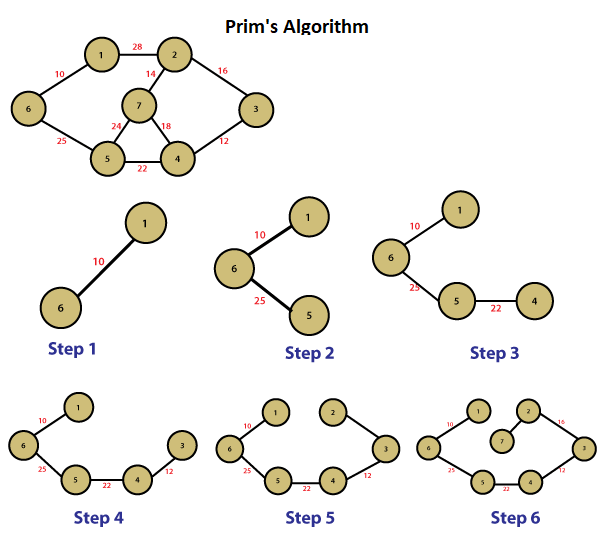
\includegraphics[width = 0.7\textwidth]{kauan_imagens/prims-algorithm-java.png}
\caption{Um grafo e sua árvore de caminho mínimo de acordo com o algoritmo de Prim}
\label{fig:enter-label}
\end{figure}


\subsection{Algoritmo de Kruskal}

Aqui trataremos do algoritmo de Kruskal para encontrar a árvore geradora mínima de um grafo dado.
No algoritmo de Kruskal, ordenamos todas as arestas pelo seu peso em ordem crescente. Assim, vamos adicionar uma aresta e seus vértices à árvore se essas não formarem ciclos com os componentes já adicionados. Primeiramente, escolhem-se as arestas de menor peso e as de maiores pesos serão adicionadas por último. Seguindo o método, podemos dizer que o algoritmo faz uma escolha ótima local em cada passo com a intenção de encontrar a solução ótima. Portanto, é um algoritmo ganancioso. 


\subsubsection{Criando árvore geradora mínima usando o algoritmo de Kruskal}

Examinemos as etapas envolvidas no Algoritmo de Kruskal para gerar uma árvore geradora mínima:

\begin{itemize}
    \item \textbf{Etapa 1:} Classifique todas as arestas em ordem crescente de seus pesos.
    \item \textbf{Etapa 2:} Escolha a menor aresta.
    \item \textbf{Etapa 3}: Verifique se a nova aresta cria um ciclo ou loop em uma árvore geradora.
    \item \textbf{Etapa 4:} Se não formar o ciclo, inclua essa aresta na MST. Caso contrário, descarte-a.
    \item \textbf{Etapa 5:} Repita a partir da etapa 2 até incluir $|V| - 1$ arestas na MST.
\end{itemize}


\begin{SCfigure}[0.5][h]
    \caption{$\left[
    \begin{array}{cccc}
    Aresta & Peso\\
    (E,F) & 2\\
    (F,D) & 2 \\
    (C,F) & 3 \\
    (B,C) & 3\\
    (C,D) & 4 \\
    (B,F) &  5\\
    (D,E) & 5\\
    (B,D) & 6\\
    (A,B) & 7\\
    (A,C) & 8
    \end{array}
    \right]$}
    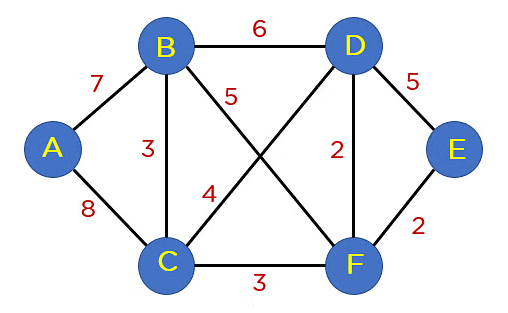
\includegraphics[width=7cm]{Kruskal/inicializacao.png}
\end{SCfigure}

\begin{figure}[htp]

\centering
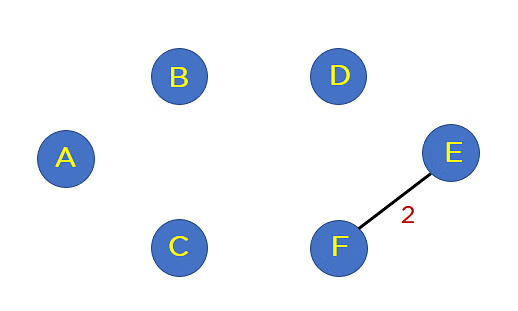
\includegraphics[width=.32\textwidth]{Kruskal/iter1.png}\hfill
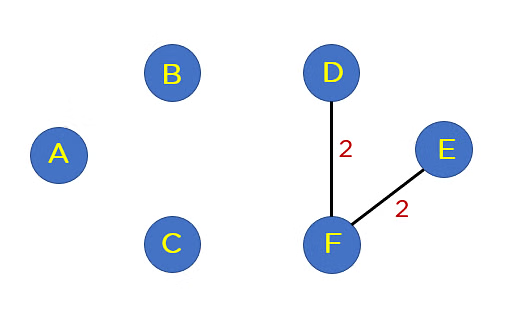
\includegraphics[width=.32\textwidth]{Kruskal/iter2.png}\hfill
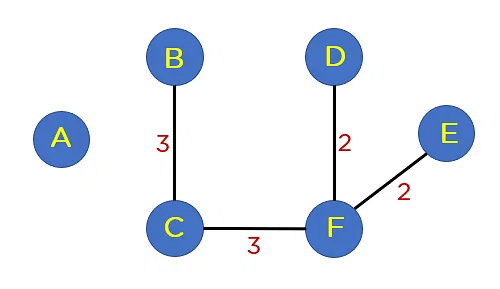
\includegraphics[width=.32\textwidth]{Kruskal/iter3.png}

\end{figure}




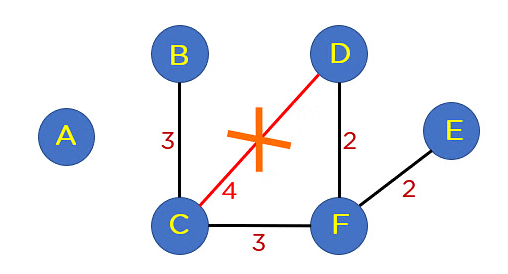
\includegraphics[width=.32\textwidth]{Kruskal/iter4.png}\hfill
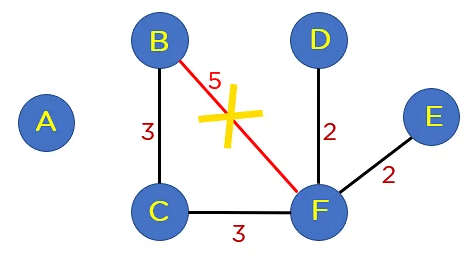
\includegraphics[width=.32\textwidth]{Kruskal/iter5.png}\hfill
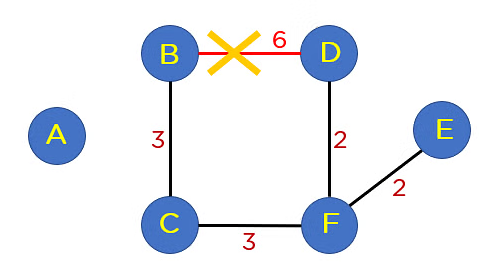
\includegraphics[width=.32\textwidth]{Kruskal/iter6.png}




\begin{figure}%
    \centering
    \subfloat[\centering Iteração 7: todos os vétices foram adicionados, então essa é a árvore resultante.]{{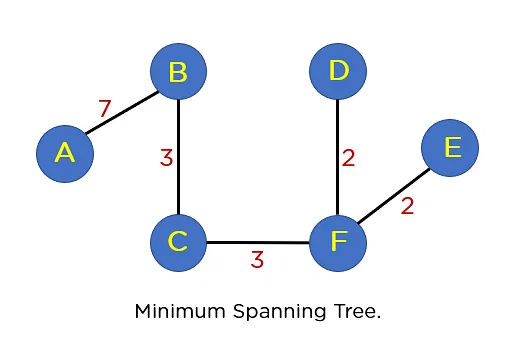
\includegraphics[width=7cm]{Kruskal/mst.png} }}%   
\end{figure}

Com isso, concluímos a construção de uma árvore geradora mínima através do algoritmo de Kruskal.

\section{Aplicando computacionalmente}

Por fim, fizemos a aplicação computacional em Python dos três algoritmos apresentados. Os notebooks podem ser encontrados no repositório do GitHub localizado \href{https://github.com/kauanmaf/trabalho_mat_discreta}{\textcolor{blue}{nesse link}}.

\section{Conclusão}
Concluimos, assim, que a necessidade de buscar caminhos mínimos em árvores, mesmo que sem todo o formalismo definido pela teoria dos grafos, é um problema recorrente na história da humanidade, e, consequentemente, a formulação de algoritmos para resolver esse problema é algo importante para a sociedade. \\

Outrossim, pode-se afirmar que é possível aplicar computacionalmente os algoritmos clássicos supramencionados, tais como o algoritmo de Borůvka, o de Prim e o de Kruskal, com apenas algumas simples classes e funções no Python. \\

Ademais, é importante ressaltar que o presente trabalho contribuiu para a nossa formação acadêmica e nos permitiu aprender mais sobre a teoria de grafos como um todo.

\vspace{2cm}

\section{Bibliografia}
[1] GRAHAM, Ronald L.; HELL, Pavol. On the history of the minimum spanning tree problem. Annals of the History of Computing, v. 7, n. 1, p. 43-57, 1985. \\

[2] RUSSELL, J.; COHN, R. Minimum Spanning Tree. 1. ed. [s.l.] Book on Demand, 2013. \\

[3] MINIMUM SPANNING TREES - BORUVKA'S ALGORITHM. \textbf{StackAbuse}. Disponível em: https://stackabuse.com/courses/graphs-in-python-theory-and-implementation/lessons/minimum-spanning-trees-boruvkas-algorithm/. Acesso em: 15 de novembro de 2023. \\

[4] PRIM'S MINIMUM SPANNING TREE (MST). \textbf{Geeksforgeeks}. Disponível em: \\ https://www.geeksforgeeks.org/prims-minimum-spanning-tree-mst-greedy-algo-5/. Acesso em: 10 de novembro de 2023. \\

[5] A. S., Ravikiran. Your One-Stop Solution to Learn Kruskal Algorithm From Scratch. \textbf{SimpliLearn}. Disponível em: https://www.simplilearn.com/tutorials/data-structure-tutorial/kruskal-algorithm. Acesso em: 18 de novembro de 2023. \\

[6] Kruskal's Minimum Spanning Tree (MST) Algorithm. \textbf{Geeksforgeeks}. Disponível em: \\ https://www.geeksforgeeks.org/kruskals-minimum-spanning-tree-algorithm-greedy-algo-2/.
Acesso em: 17 de novembro de 2023. \\

[7] LAHIRI, Neelakshi. Introduction and Properties of Minimum Spanning Tree. \textbf{Coding Ninjas}. Disponível em: https://www.codingninjas.com/studio/library/introduction-and-properties-of-minimum-spanning-tree. Acesso em: 17 de novembro de 2023.


\end{document}